%==== Document Setup (usthesis)======================================
\documentclass[masters-a,                       %... Document type
               12pt,oneside,openany,a4paper, %... Layout
               a5block,                      %... A5 type block
              afrikaans ,english,           %... Afrikaans default language
               ]{usthesis}

\usepackage{siunitx}
\usepackage{lipsum} 
\usepackage{graphicx}% http://ctan.org/pkg/graphicx
\usepackage{multirow}% http://ctan.org/pkg/multirow
\usepackage{booktabs}% http://ctan.org/pkg/booktab
\usepackage{amssymb}
\usepackage{subcaption}
%
% PLEASE read the USthesis documentation for the class options
% and how to set line and paragraph spacing
%

%==== Math setup ====================================================
 \usepackage{amsmath}%............................ Advanced math (before fonts)
 %\usepackage{amssymb}%............................ AMS Symbol fonts

%==== Font setup (default is Computer Modern) =======================
 \usepackage[T1]{fontenc}%........................ Type 1 fonts
 \usepackage{textcomp}%........................... Additional text character
 \usepackage{bm}%................................. Bold math symbols (after fonts)

%==== Ref's, Bib's and Nomencl ======================================
 \usepackage{usnomencl}%.......................... List of symbols (in usthesis pack)

 \usepackage{usbib}%.............................. Bibliography    (in usthesis pack)
    \bibliographystyle{usmeg-n}
    \renewcommand\bibfont{\small}
    %% For usmeg-a, the bib is a list of references. If you
    %% are using usmeg-n comment out the following lines

    \renewcommand{\bibname}{References} 

%==== Graphics and Color ============================================
\usepackage{graphicx}%........................... Graphicx loaded in usthesis
\usepackage{color}%.............................. Color setup

%==== Additional USthesis packages ==================================

\usepackage{ussummary}%.......................... Mech Eng summary page (in usthesis pack)

%==== Local Defs ====================================================
\makeatletter


\makeatother
%==== Title Page ====================================================

\title{Report for E-design 344}

\author{Alex mUthua}
       {Alex Muthua\\
           21317682}

\subject{E-Design 344}
        {}

\ReportDescript{E-Design report \# \textcolor{red}{2}}

\address{Departement of Electrical and Electronic Engineering,\\
         Universiteit van Stellenbosch,\\
         Privaatsak X1, Matieland 7602.}

%\studyleader{Name of supervisor}

\setdate{\today}

%====================================================================%
%                 T H E   M A I N   D O C U M E N T                  %
%====================================================================%
\begin{document}

\frontmatter%========================================================

\TitlePage
\chapter{Declaration}

By submitting this report electronically, I declare that the entirety of the work contained
therein is my own, original work, that I am the sole author thereof (save to the extent
explicitly otherwise stated), that reproduction and publication thereof by Stellenbosch
University will not infringe any third party rights and that I have not previously in its
entirety or in part submitted it for obtaining any qualifcation.

\vspace{3cm}
\hspace{2cm}
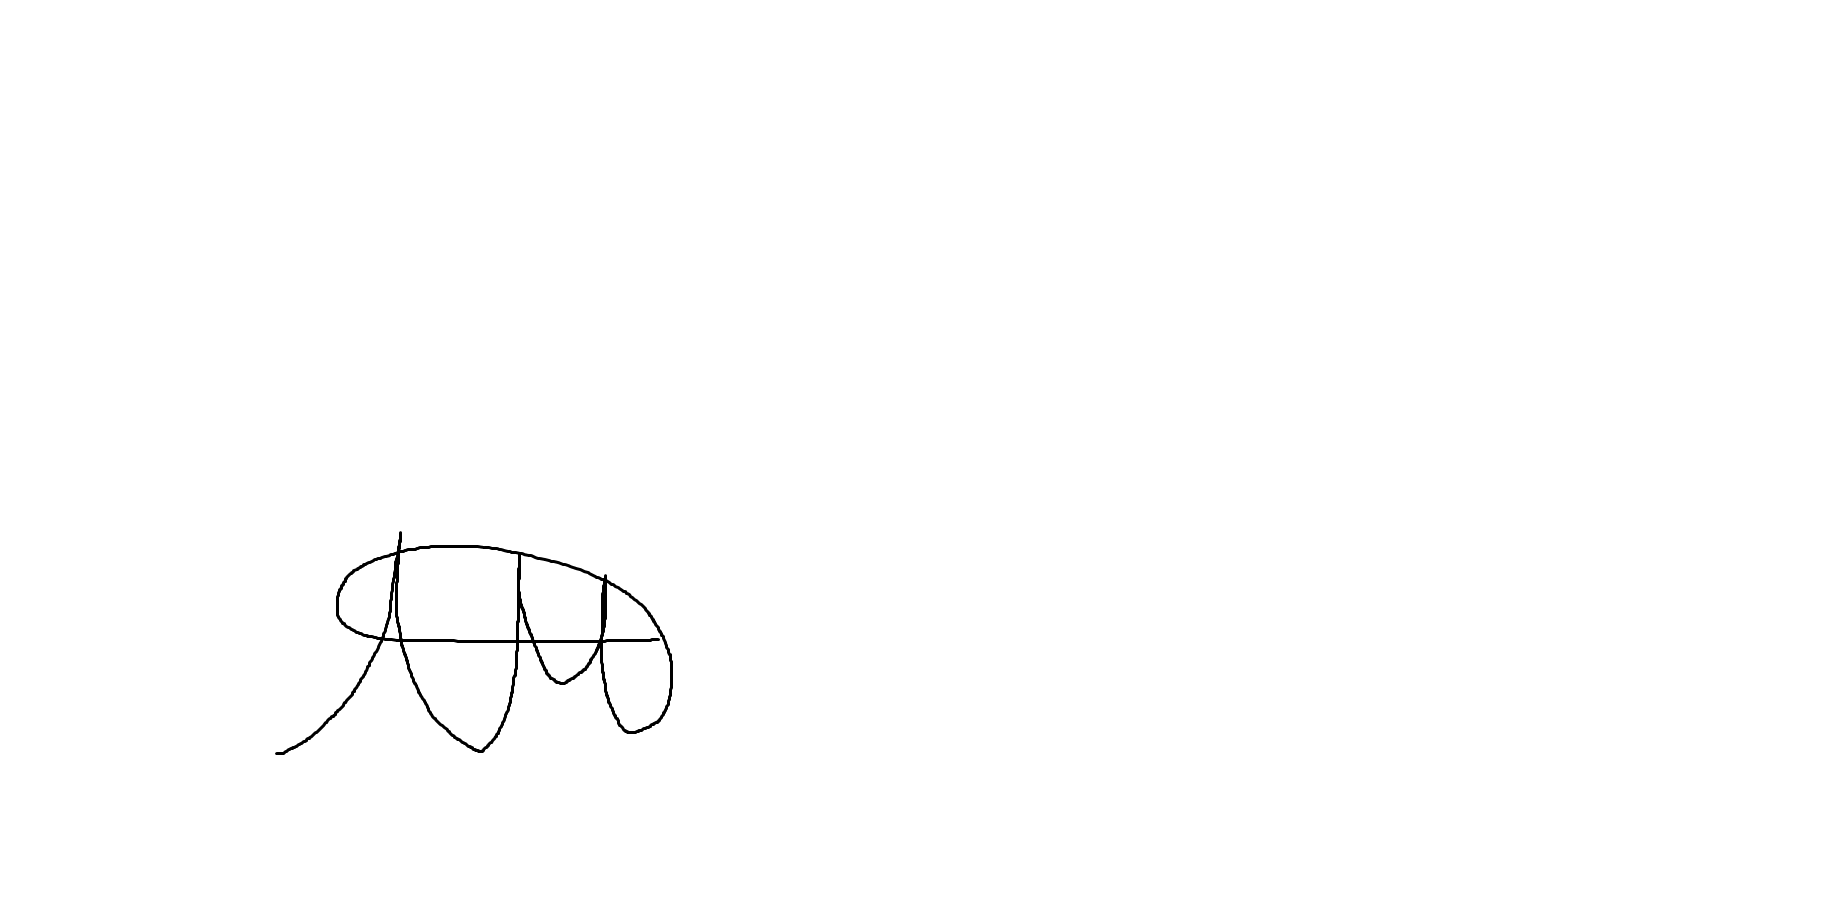
\includegraphics[width=0.4\linewidth]{./Figures/Signature-Alex.png}\\
\noindent%
\parbox{.5\textwidth}{%
  Signature:\quad\dotfill\par
  \hfill A.\ Muthua\hspace{1.2cm}\null}


\vspace{1.2cm}
\hspace{2cm}
\today \\
\noindent%
\parbox{.5\textwidth}{%
  Date:\quad\dotfill\par}

\tableofcontents
\listoffigures
\listoftables
\chapter{Nomenclature}

\begin{Nomencl}
 \NomGroup{Constants}%-----------------------------------------------
   \item[$\mathrm{g} = $] $\mathrm{9.81\,m/s^2}$

 \NomGroup{Variables}%-----------------------------------------------
   \item[$C$] \UnitLine{Capacitance}{F}
   \item[$Q$] \UnitLine{Charge}{C}
   \item[$i$] \UnitLine{Current}{A}
   \item[$P$] \UnitLine{Power}{W}
   \item[$R$] \UnitLine{Resistance}{$\Omega$}
   \item[$\Theta$] \UnitLine{Thermal resistance}{^oC/W}
   \item[$V$] \UnitLine{Voltage}{V}

 \NomGroup{Abbreviations}%-----------------------------------------------
   \item[BJT] \quad\dotfill Bipolar Junction Transistor
   \item[MOSFET] \quad\dotfill Metal Oxide Semiconductor Field Effect Transistor
   \item[AC]  \quad\dotfill Alternating Current
   \item[DC]  \quad\dotfill Direct Current
   \item[ADC]  \quad\dotfill Analog-to-Digital Converter
   \item[op-amp]  \quad\dotfill Operational Amplifier
   \item[XOR]  \quad\dotfill Exclusive Or Logic Gate
   \item[PWM]  \quad\dotfill Pulse-Width Modulation

\end{Nomencl}


\endinput


\mainmatter%=========================================================

\chapter{Signal conditioning system design}
\section{System overview} \label{sec:system}
\begin{figure}
    \centering
    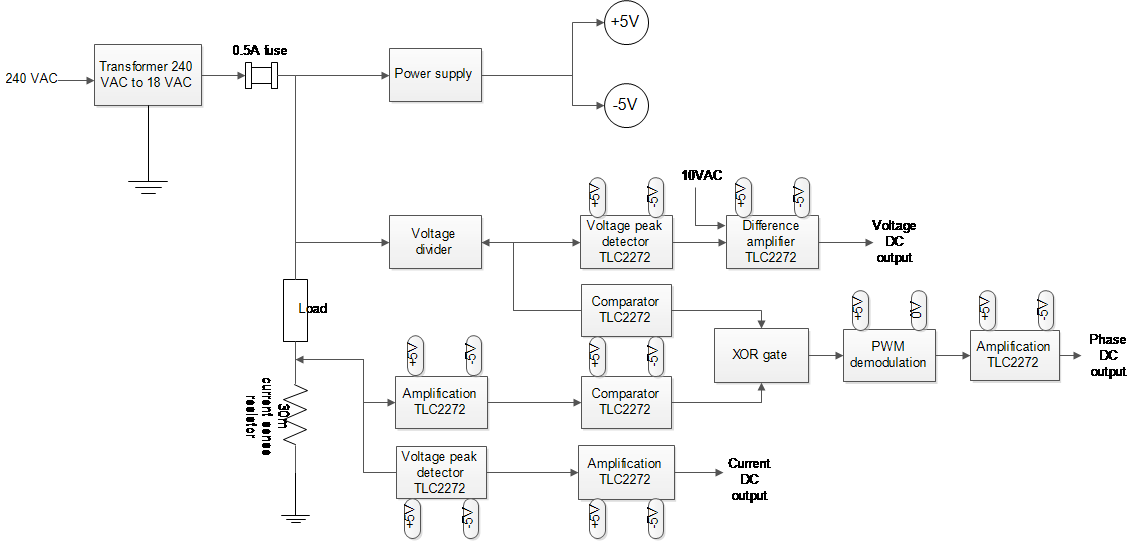
\includegraphics[width = 1\linewidth]{Figures/system_overview_2}
    \caption{System diagram}
    \label{fig:system_diagram}
\end{figure}

The TLC2272 rail-to-rail op amps were selected for all three transducers. This is due to their compact nature (2 op amps in one package as compared to the 1:1 ratio of the TL081), as well as their ability to produce output voltages much closer to the rails, which improves the resolution of the final values.
Each TLC2272 op amp draws approximately $2.4\SI{\milli}{\ampere}$\cite{TLC2272} from the $\pm5\si{\volt}$ supplies. As the system uses 8 op-amps, as well as an XOR gate, this amounts to a draw of approximately $\SI{20}{\milli\ampere}$. This is well within the specification they were designed for.










\chapter{Rectifier}
\section{Theory and related work} \label{sec:literature_rectifier}
A basic half-wave rectifier consists of a diode in series with a sinusoidal input voltage. This allows only the positive cycle of the input to appear at the output. Adding a shunt/filter capacitor to the rectifier's output allows for current to flow continuously as the capacitor discharges during the cutoff period of the diode \cite{Neamen:Microelectronics}.


\section{Design} \label{sec:design_rectifier}

\textbf{\textit{Design rationale}} \\
For this design, the main consideration is that the capacitor is large enough to supply current to the rest of the circuit at the required voltage. This is calculated in Equation \ref{eq:rectifier_capacitor}. However, the current flowing through the diode is also a concern as a \SI{0.5}{\ampere} fuse is installed in the design. So, it must be ensured that any transient charging currents are not large or sustained enough that the fuse blows. The 1N4007 diode used here has a peak reverse voltage of \SI{700}{\volt}\cite{1N4007} which is more than sufficient.


\noindent\textbf{\textit{Design calculations}} \\
\textit{Capacitor calculation:}
\begin{equation}\label{eq:rectifier_capacitor}
\begin{split}
        dQ &= i \times dt = C(V_{pk} - V_{min}) \\ 
        C &= \frac{\SI{200}{\milli\ampere} \times 0.02}{\SI{18}{\sqrt{2}}-0.7-12} = \SI{313.6}{\mu\farad}
\end{split}
\end{equation}
Ideally, a $\SI{330}{\mu\farad}$ capacitor would be used. However, due to the voltage rating of the available capacitors, two $\SI{220}{\mu\farad}$ capacitors were instead used.

\textit{Diode current\cite{Neamen:Microelectronics}:}
\begin{equation}
\begin{split}
    i_{D,peak} &= i_{load}(1 + \pi\sqrt{\frac{2V_M}{V_r}})
    = \SI{200}{\milli\ampere} \times (1 + \pi\sqrt{\frac{2(18\sqrt{2}-0.7)}{18\sqrt{2}-0.7-12}}) \\
    &= \SI{1.438}{\ampere}
\end{split}
\end{equation}

This is higher than the fuse rating. However, the melting time of the fuse at this current is: $ \frac{0.215}{1.438^2} = \SI{104}{\milli s}$\cite{Fuse}. This is much higher than the maximum positive cycle period of 10ms. Hence, it can be assumed to be safe enough.


\noindent\textbf{\textit{Circuit diagram}}
\begin{figure}[h]
    \centering
    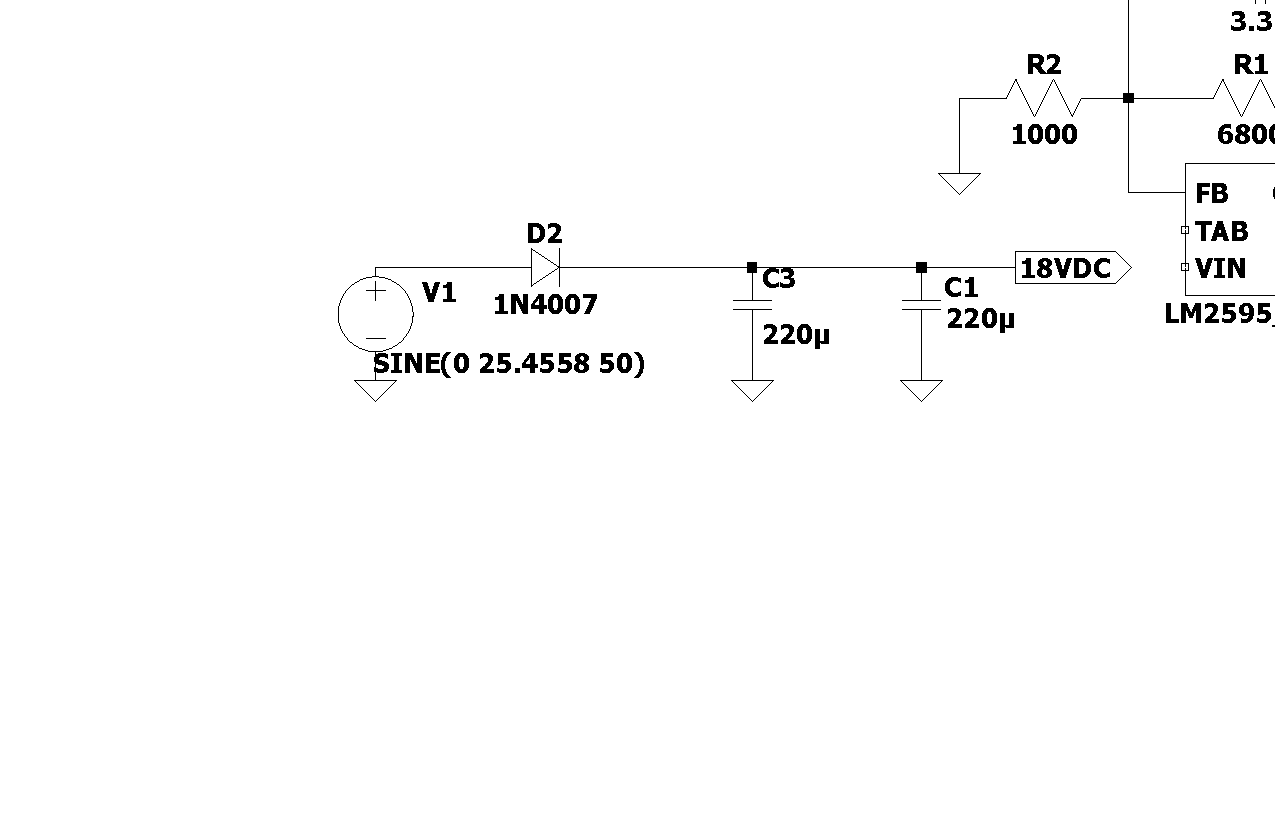
\includegraphics[clip, trim = 3cm 7cm 2cm 3.7cm,width = 0.75\linewidth]{Figures/rectifier_circuit.pdf}
    \caption{Half wave rectifier circuit}
    \label{fig:rectifier_circuit}
\end{figure}


\section{Simulation} \label{sec:simulation_rectifier}

\begin{figure}[h] 
 \centering
 
    \begin{subfigure}[]{0.5\linewidth}
        \centering
        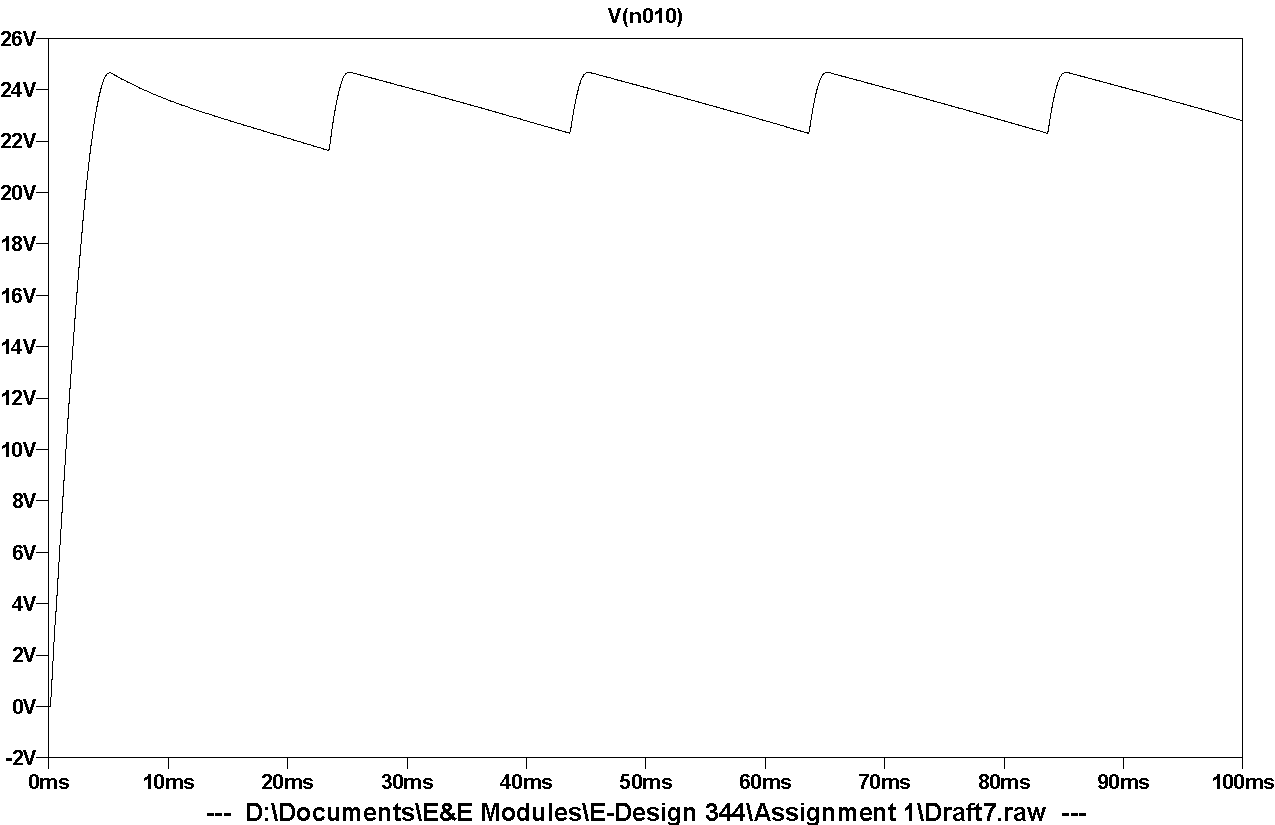
\includegraphics[width=1.\linewidth]{./Figures/rectifier_simulate.pdf}
        \caption{Simulated rectifier output.}
        \label{fig:rectifier_simulation}
    \end{subfigure}
    \begin{subfigure}[]{0.44\linewidth}
        \centering
        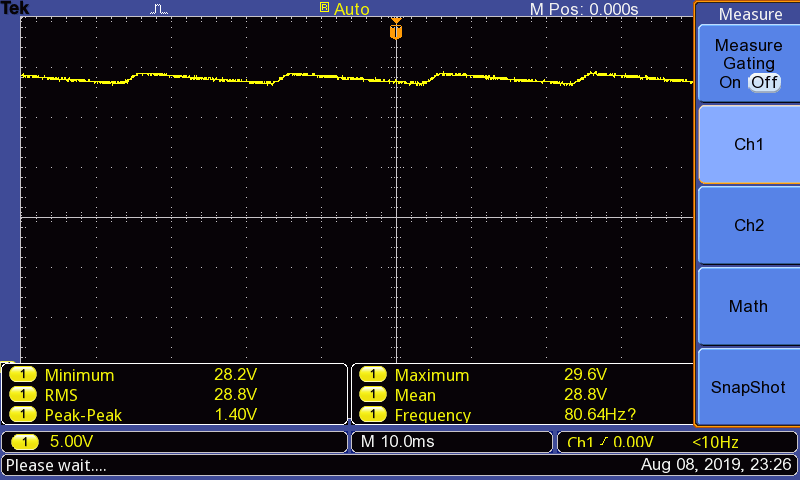
\includegraphics[width=1.\linewidth,clip,trim = 0.3cm 0cm 2.5cm 0cm]{./Figures/rectifier_test}
        \caption{Measured rectifier output.} 
	    \label{fig:rectifier_measurement}
    \end{subfigure}
    
\caption{Rectifier simulated and measured output}
\end{figure}

\section{Measurements} \label{sec:measurements_rectifier}




\chapter{Switchmode regulation}
\section{Theory and related work} \label{sec:literature_switchmode}

Switchmode regulators operate by rapidly switching an energy storage device on and off. The duty cycle and frequency of the switch sets how much charge is transferred to the load. This, in turn determines the output voltage of the regulator. These regulators can be used to step down(buck) or step up(boost) a given input voltage. The series storage device is usually either fully conducting or switched off, thus, the regulator tends to dissipate almost no power. This gives it quite a high efficiency. Due to the switching operation of the regulator, it produces a significant ripple voltage at its output. However, it is a much better choice if the input voltage is much higher than the output voltage \cite{regulators-main}.


\section{Design} \label{sec:design_switchmode}
\textbf{\textit{Design rationale}} \\
As explained in Section \ref{sec:rationale_system}, the switchmode regulator is used to give an intermediate voltage of that is then passed through the linear regulator designed in Section \ref{sec:design_linear}. This intermediate voltage is also used to power the charge pump scheme in Section \ref{sec:design_chargepump}. The intermediate voltage is chosen as \SI{9.5}{\volt} as shown to be sufficient in Section \ref{sec:design_chargepump}.

In terms of the design of the regulator, the device's datasheet provides a sufficient circuit that is implemented in the design \cite{LM2595}.The components listed below and shown in Figure \ref{fig:switchmode_circuit} are all chosen based of \cite{LM2595}, which provides the appropriate values to use for a wide reange of applications.

\begin{itemize}
    \item A low ESR capacitor is required at the input pin to prevent large voltage transients from appearing, and to provide the instantaneous current required each time the switch turns on.
    \item A feedforward capacitor adds lead compensation to the feedback loop and increases
    the phase margin for better loop stability.
    \item An output capacitor is required to filter the output and provide regulator loop stability. Low impedance/ ESR capacitors designed for switching regulator applications must be used.
    \item Buck(step-down) regulators require a diode to provide a return path for the inductor current when the switch turns off. Because of their very fast switching speed and low forward voltage drop, Schottky diodes provide the best performance.
    \item An inductor at the output is used to store energy such that current continuously flows, even when the regulator is "switched off". An inductor of $\SI{330}{\mu H}$ is suggested, but a smaller inductor is already provided. So, it is used as it will provide just as much or more continuous current.
    \item Resistors, R1 and R2 in Figure \ref{fig:switchmode_circuit}, are used to adjust the output voltage as shown in Equation \ref{eq:switchmode_output}.
    
\end{itemize}


\noindent\textbf{\textit{Design calculations}} \\
\textit{Feedback resistors/ Adjusting voltage output \cite{LM2595}:}
\begin{equation} \label{eq:switchmode_output}
    \begin{split}
        V_{out} &= (1+\frac{R_1}{R_2})V_{ref} \\
        R_1 &= R_2(\frac{V_{out}}{V_{ref}}-1) 
        = 1k(\frac{9.5}{1.23}-1) \\
        &=\SI{6.724}{\kilo\ohm}
    \end{split}
\end{equation}
A $\SI{10}{\kilo\ohm}$ variable resistor is placed at $R_1$ and set to give the required output voltage.


\noindent\textbf{\textit{Circuit diagram}}
\begin{figure}[h!]
 \centering
  	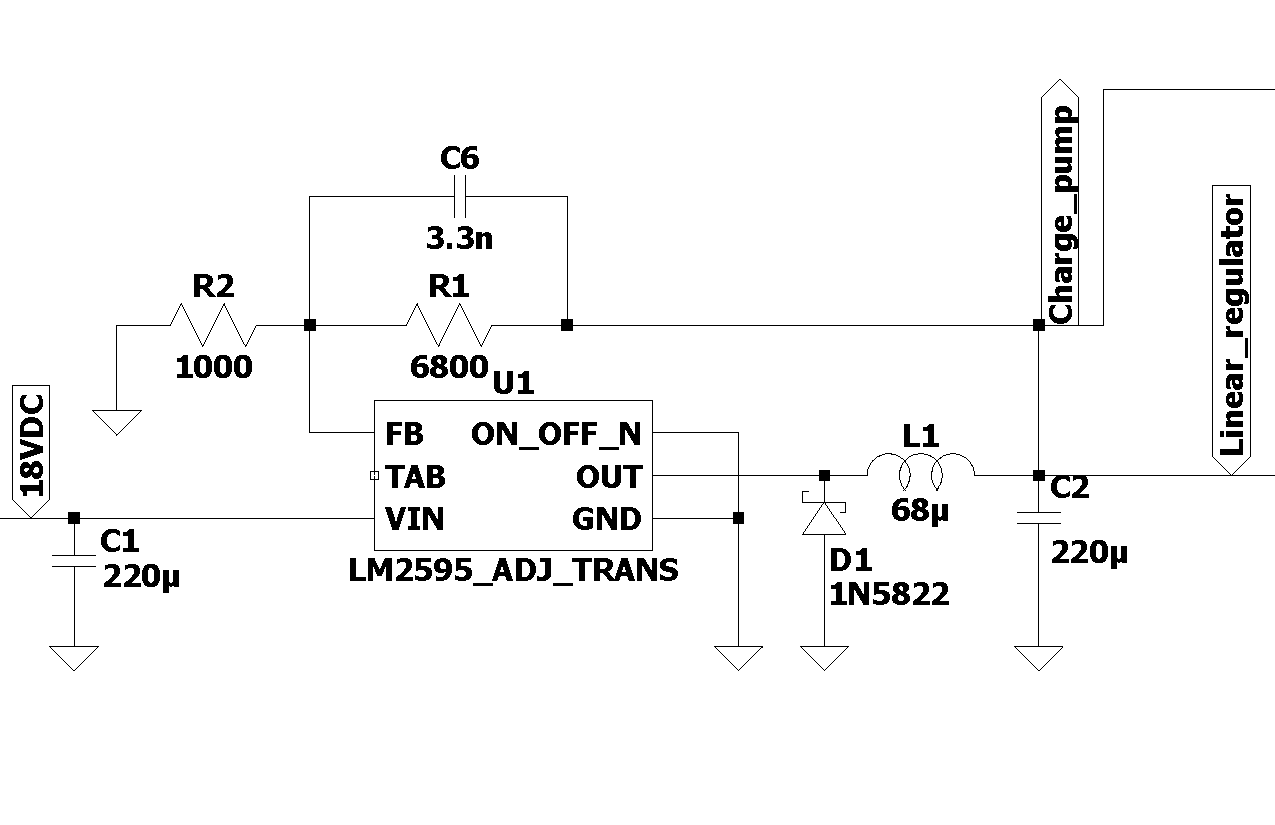
\includegraphics[width=0.55
  	\linewidth,clip,trim = 0cm 2.5cm 0cm 1cm]{./Figures/switchmode_circuit.pdf}
  	\caption{Switchmode regulator circuit.}
  	\label{fig:switchmode_circuit}
 \end{figure}


\section{Simulation} \label{sec:simulation_switchmode}
A plot of the LTSpice switchmode regulator simulation is given in Figure \ref{fig:switchmode_simulation}.
\begin{figure}[h] 
 \centering
  	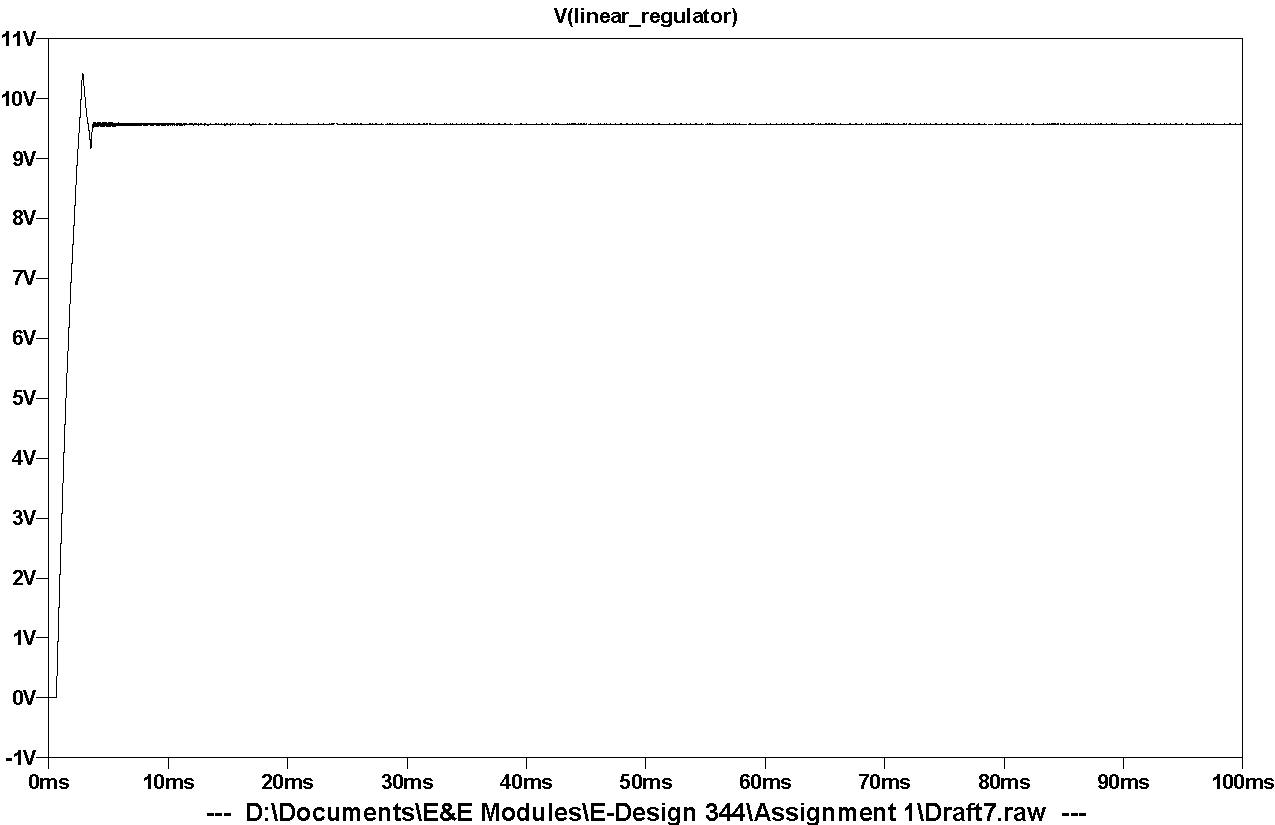
\includegraphics[width=0.7\linewidth]{./Figures/switchmode_simulate.pdf}
  	\caption{Simulated switchmode output.}
  	\label{fig:switchmode_simulation}
 \end{figure}
 
 
\section{Measurements} \label{sec:measurements_switchmode}
The measured output voltage from the switchmode is given in Figure \ref{fig:switchmode_measurement_box}.
\begin{figure}[h]
 \centering
        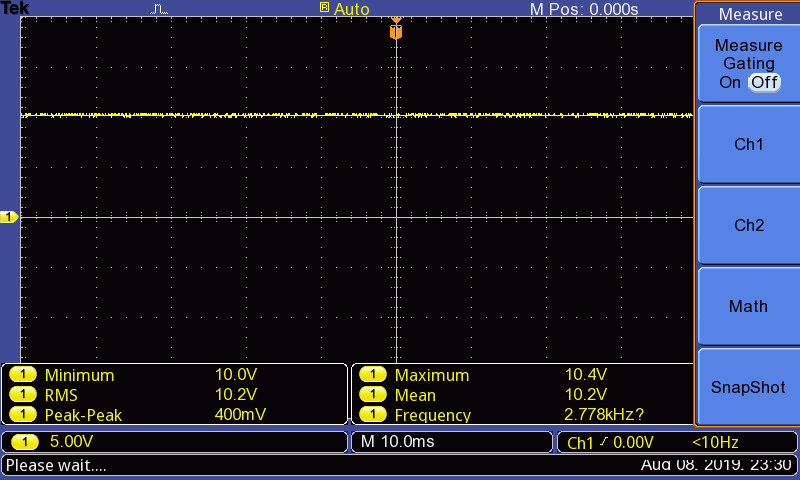
\includegraphics[width=0.6\linewidth,]{./Figures/switchmode_test}
        \caption{Switchmode output voltage}
\caption{Switchmode measured output}
\label{fig:switchmode_measurement_box}
\end{figure}








\chapter{Phase shift transducer}
\section{Theory and related work} \label{sec:literature_phase}
A phase shift transducer converts the phase shift between two signals to an analog DC output.  For the purpose of this project, an XOR-gate based phase detector is used to implement this transducer. The presence of a phase shift between two signals introduces an equivalent time delay between them. An XOR gate produces a logical high when its two inputs have different logical states, which would occur during this time delay. The resultant output is a square signal with a duty cycle equal to the time shift between the two original signals. Thus, the width of the pulse of the output signal changes proportionally to the phase difference between the input signals and is said to be pulse-width modulated (PWM)\cite{phase_detector}. The XOR phase detector can only be used for phase shifts of $\numrange{0^o}{180^o}$, thus, it is sufficient for this project.

Since the input signals (voltage and current) are sinusoidally varying, they must be modified before being supplied to the XOR gate. To obtain the required digital signals, a comparator can be used. By having the same reference for both comparators, the XOR inputs will be offset by the same time delay as the sinusoidal signals as required. 

However, the XOR phase detector outputs a digital signal. To convert this to an analog value, a demodulator for the PWM signal must be considered. The simplest of these is a low pass RC filter\cite{pwm_low_pass}. By setting the RC constant to be much larger than the PWM signal period, the filter acts as an integrator. Its output is then the average of the XOR gate output signal. The behaviour of the phase transducer can thus be described as: $V_{out} = V_{DD} \times \frac{\Delta\Theta}{180^o}$\cite{phase_detector}

Since the range of the phase detector is up to $180^o$, the resolution may be impacted. To improve this an amplification stage is added to map $45^o$ closer to the maximum range. While this would cause clipping for higher phase shifts, it is not a major concern given this project's specifications. A standard non-inverting amplifier, as shown in Figure \ref{fig:non_invert_amp} can be used for this.

\section{Design} \label{sec:design_phase}
The design of the transducer begins with the two comparators for the voltage and input signals. The TLC2272 op-amps are chosen for this, as they produce sufficiently high voltage, so as to be seen as a logical high by an XOR gate\cite{XOR}. The reference for both is also chosen to be $\SI{0}{\volt}$ as it is easily obtained by connecting to the ground plane. The voltage signal to the comparator must first be scaled down to be within the common-mode and input voltage limits of the op-amp. Equation \ref{eqn:voltage_divider} shows the ratio of the voltage divider to be used for this purpose. The same voltage divider is used for the input of the voltage comparator as it complies with the common-mode, differential and input limits as shown in Section \ref{sec:design_voltage}. 

For the current signal comparator, it is considered that the current sense resistor provides extremely low voltages.Some of these are even less than the op-amp's input offset voltage and would therefore affect the comparator's performance. A non-inverting amplifier is therefore designed to amplify the signal to a more usable range. An amplifier for the current signal had been designed in Section \ref{sec:design_current}, but combined with a precision rectifier. Isolating just the amplifier gives a signal that should conform  to the limits(common-mode, differential and input voltages) of the op-amp used for the comparator as previously shown. 

It is however observed during simulation, that the non-inverting amplifier introduces a small DC offset, such that the amplified signal is no longer centred around $\SI{0}{\volt}$. So, the current comparator setup would not provide the required output. To counteract this, the amplified signal is measured and found to be centred around $\SI{54}{\milli\volt}$. The inverting input of the op-amp is thus connected to a voltage approximately equal to this by passing the +5V supply through a voltage divider circuit. Selecting a $\SI{100}{\kilo\ohm}$ and $\SI{1}{\kilo\ohm}$ resistor gives: $V_{ref} = \frac{1\si{\kilo}}{1\si{\kilo}+100\si{\kilo}} \times 5 = \SI{49.5}{\milli\volt}$. As this value may vary from op-amp to op-amp, a $\SI{1}{\kilo\ohm}$ potentiometer is chosen for the final design, so that it can be manually tuned in practice.

As the XOR gate can only handle voltages greater than $\SI{-0.5}{\volt}$ at its input\cite{XOR}, the outputs of the comparator are passed through a diode before the gate. The XOR gate is then supplied with the previously designed $\SI{+5}{\volt}$ supply.

As explained before, the RC filter must have a RC constant much larger than the PWM signal period. This also has the upside of reducing the ripple voltage at its output. However, making this constant too large increases the settling time of the filter, thus, a balance between the two must be achieved. Selecting a $\SI{1}{\mu\farad}$ capacitor, the resistor can be calculated to be: $RC > 10 \times T = 0.1$. Thus the resistor should be larger than $\SI{100}{\kilo\ohm}$. A $\SI{470}{\kilo\ohm}$ potentiometer is used in this place and tuned accordingly in practice, so as to balance the above mentioned trade-off.


For the maximum specification of $45^o$, the phase detector gives an output of 1.25V. The gain of the non-inverting amplifier is chosen such that this is mapped to 4.5V, which is sufficiently close to the rails. This gives a gain of 3.6. Choosing resistors as $\SI{5.6}{\kilo\ohm}$ and $\SI{2.2}{\kilo\ohm}$ gives: $1+\frac{4.7k}{2.2k} = 2.14$.

As a 10-bit ADC is to be used, the resolution is given as 4.883mV/bit. Reversing this to the input of the transducer gives a resolution of $\SI{6.227}{\mu}$s/bit or $0.1121^o$/bit.

The complete phase shift transducer circuit is given in Figure \ref{fig:phase_circuit}.

\begin{figure}
        \centering
         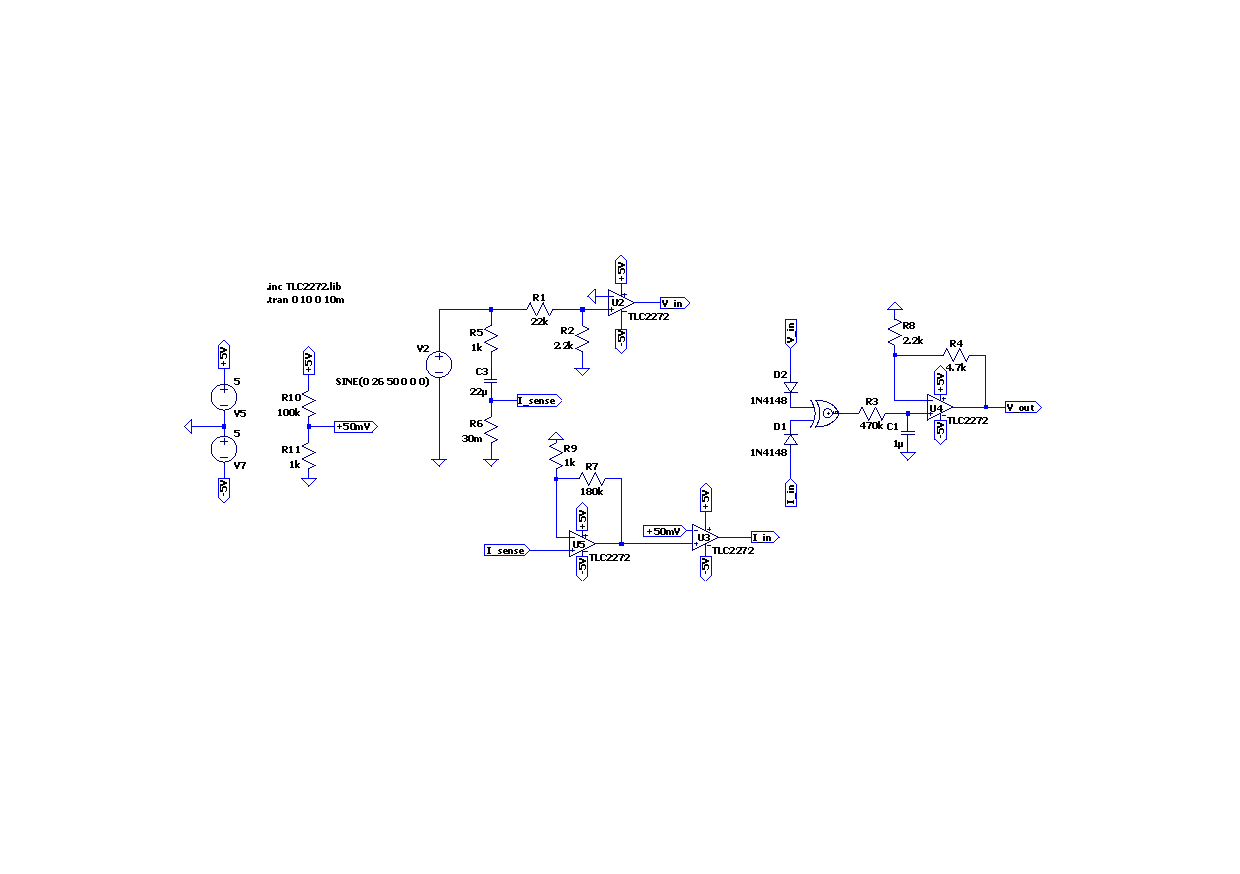
\includegraphics[width=1.15\linewidth,clip, trim = 3cm 3cm 0cm 3cm]{./Figures/phase_circuit.pdf}
		    \caption{Phase shift transducer circuit.} \label{fig:phase_circuit}
 \end{figure}

\section{Simulation} \label{sec:simulation_phase}

\begin{figure}[h] 
 \centering
 
    \begin{subfigure}[]{0.65\linewidth}
        \centering
        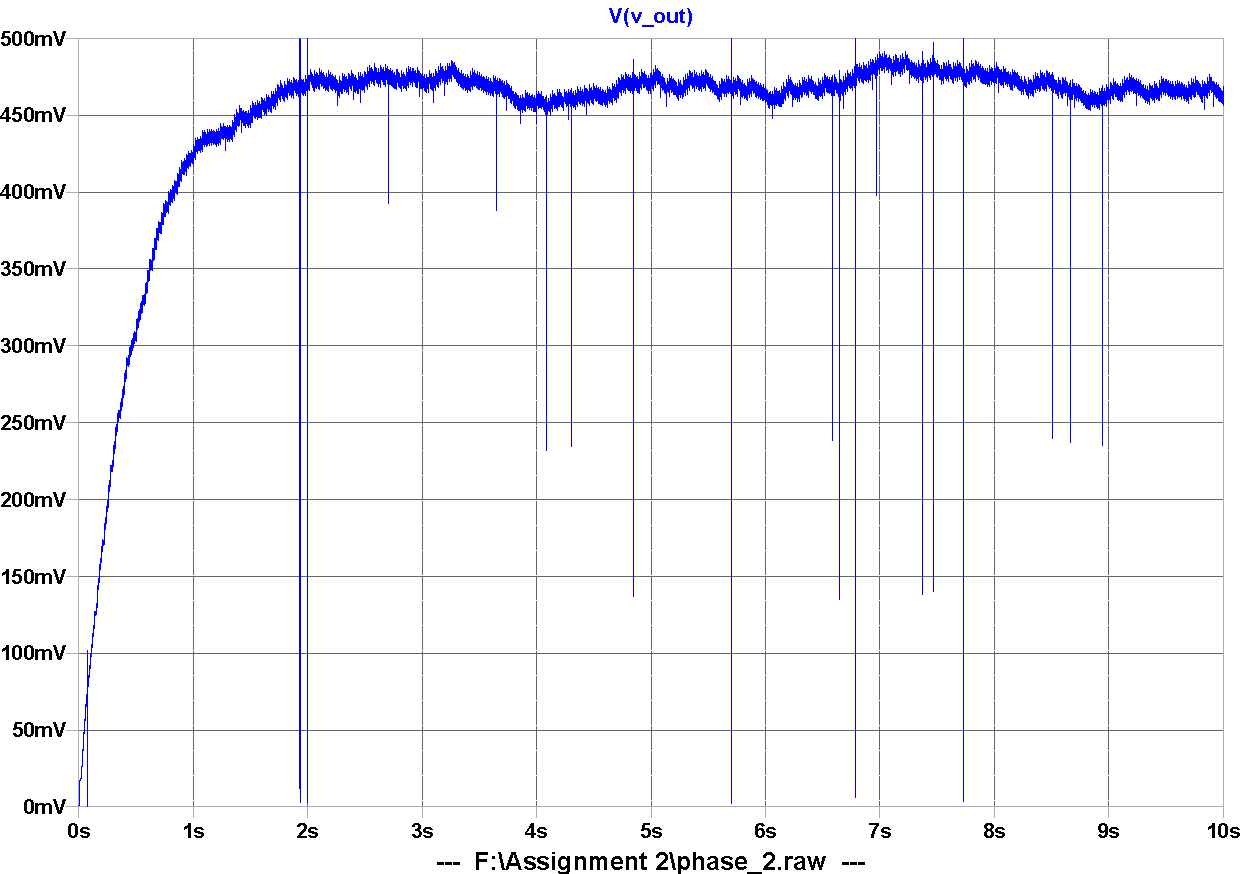
\includegraphics[width=1.\linewidth]{./Figures/phase_transducer_simulation_22u.pdf}
        \caption{$\SI{1}{\kilo\ohm}$ and $\SI{22}{\mu\farad}$ load.}
        \label{fig:phase_simulation_22u}
    \end{subfigure}
    \begin{subfigure}[]{0.65\linewidth}
        \centering
        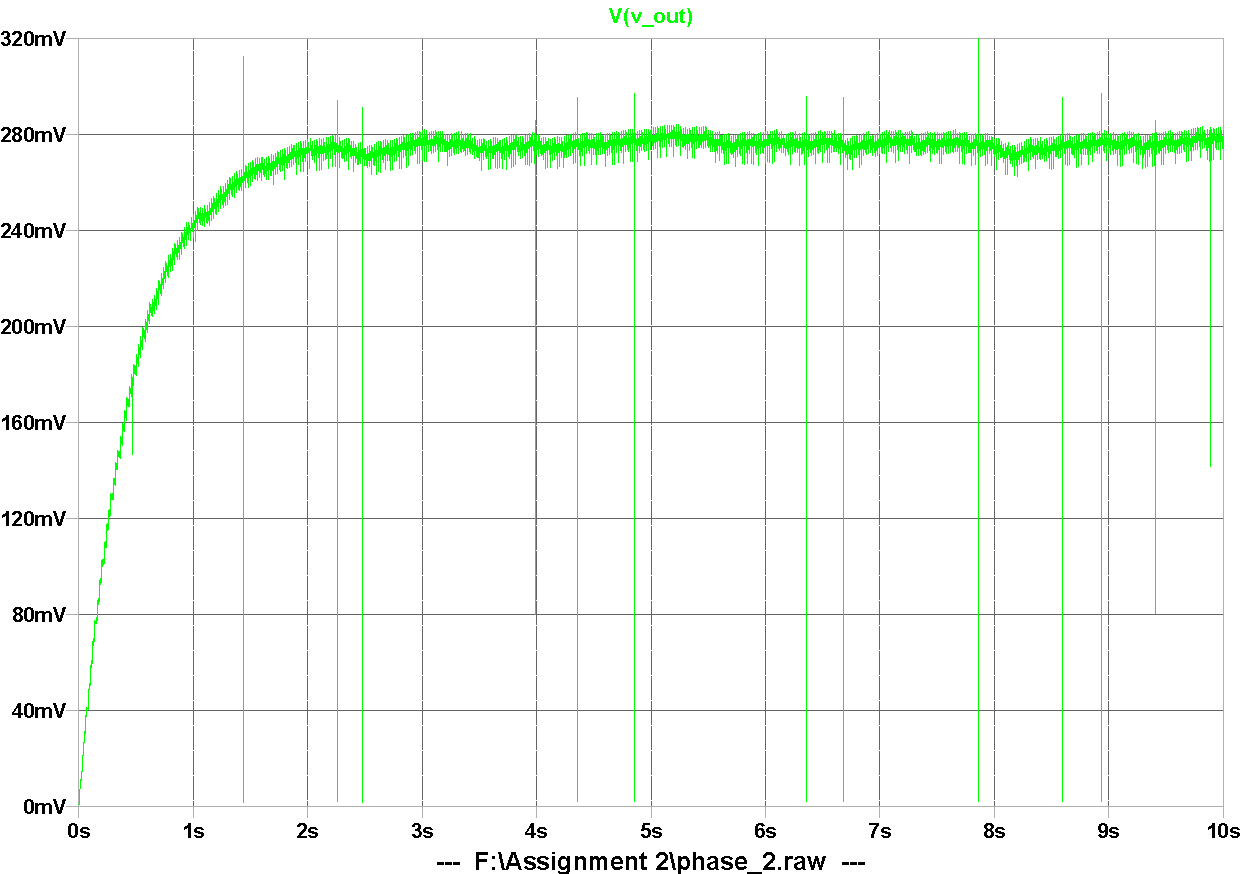
\includegraphics[width=1.\linewidth]{./Figures/phase_transducer_simulation_33u.pdf}
        \caption{$\SI{1}{\kilo\ohm}$ and $\SI{33}{\mu\farad}$ load.}
	    \label{fig:phase_simulation_33u}
    \end{subfigure}
    
\caption{Phase shift transducer simulation for nominal loads.}
\end{figure}

\section{Measurements} \label{sec:measurements_phase}
The conversion in Table \ref{tab:phase_integrated_test} is derived from the circuit in Figure \ref{fig:phase_circuit}.

$V_{out} = (1 + \frac{4.7k}{2.2k}) \times 5 \times \frac{\Delta\Theta}{180^o} = \Delta\Theta(0.08712)$
\begin{figure}
 \centering
     \begin{subfigure}[]{0.45\textwidth}
        \centering
         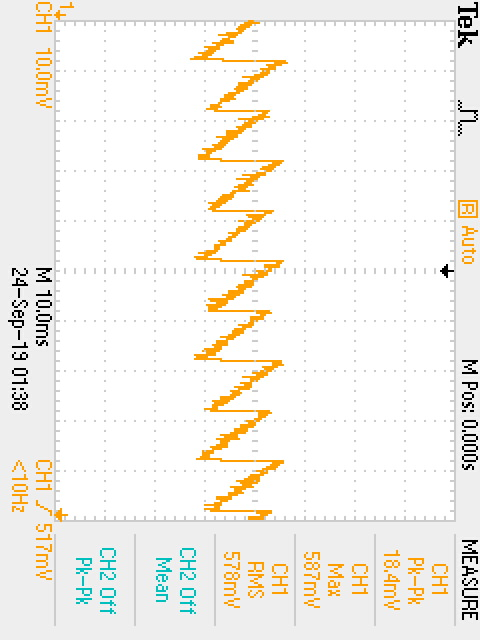
\includegraphics[height=1\linewidth,angle =90]{./Figures/phase_measure}
		    \caption{AC input and DC output for mid range load.} \label{subfig:phase_measure}
     \end{subfigure}
      \begin{subfigure}[]{0.45\textwidth}
              \centering
  		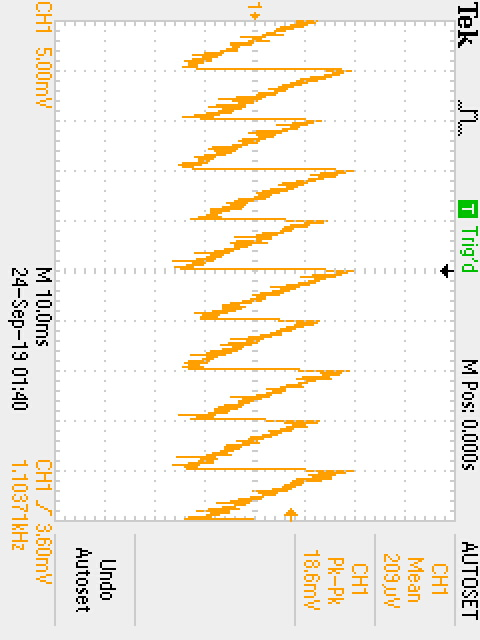
\includegraphics[height=1\linewidth,angle=90]{./Figures/phase_noise_measure}
		    \caption{Voltage transducer noise levels for a mid sized load.} \label{subfig:phase_noise}
     \end{subfigure}
 \end{figure}

\begin{table}[h]
        \centering
        \footnotesize
        \caption{Phase shift transducer unit test results}
         \begin{tabular}{p{1.8cm}p{1.3cm}p{1.3cm}p{1.5cm}p{1.5cm}p{1.8cm}p{1.8cm}p{1.8cm}}
          \toprule
             \textit{\footnotesize Measurement} & \textit{\footnotesize Load R} & \textit{\footnotesize Load C} & \textit{{\footnotesize Measured shift}} & \textit{{\footnotesize Applied shift}} & \textit{{\footnotesize Analogue output}} & \textit{\footnotesize Conversion} & \textit{\footnotesize Difference}\\
             & $[\si{\ohm}]$ & $[\si{\mu\farad}]$ & $[ms]$ & $[^o]$ & $[\si{\volt}DC]$ & $[^o]$ & $[^o]$ \\
          \midrule
          No phase shift & 1k & none & 0.036 & 0.648 & 0.173 & 1.986 & 1.338 \\
          Max phase shift & 1k & 3.3 & 1.92 & 34.56 & 2.834 & 32.53 & 2.03 \\
          Mid range & 1k & 22 & 0.458 & 8.244 & 0.608 & 6.9788 & 1.265 \\
          Mid + $\delta$ & 1k & 33 & 0.286 & 5.148 & 0.335 & 3.845 & 1.303 \\
          Mid + $2\delta$ & 1k & 47 & 0.196 & 3.528 & 0.1806 & 2.073 & 1.455 \\
          \bottomrule
        \end{tabular}
     \label{tab:phase_integrated_test}
\end{table}








\chapter{System tests}
\begin{figure}
        \centering
         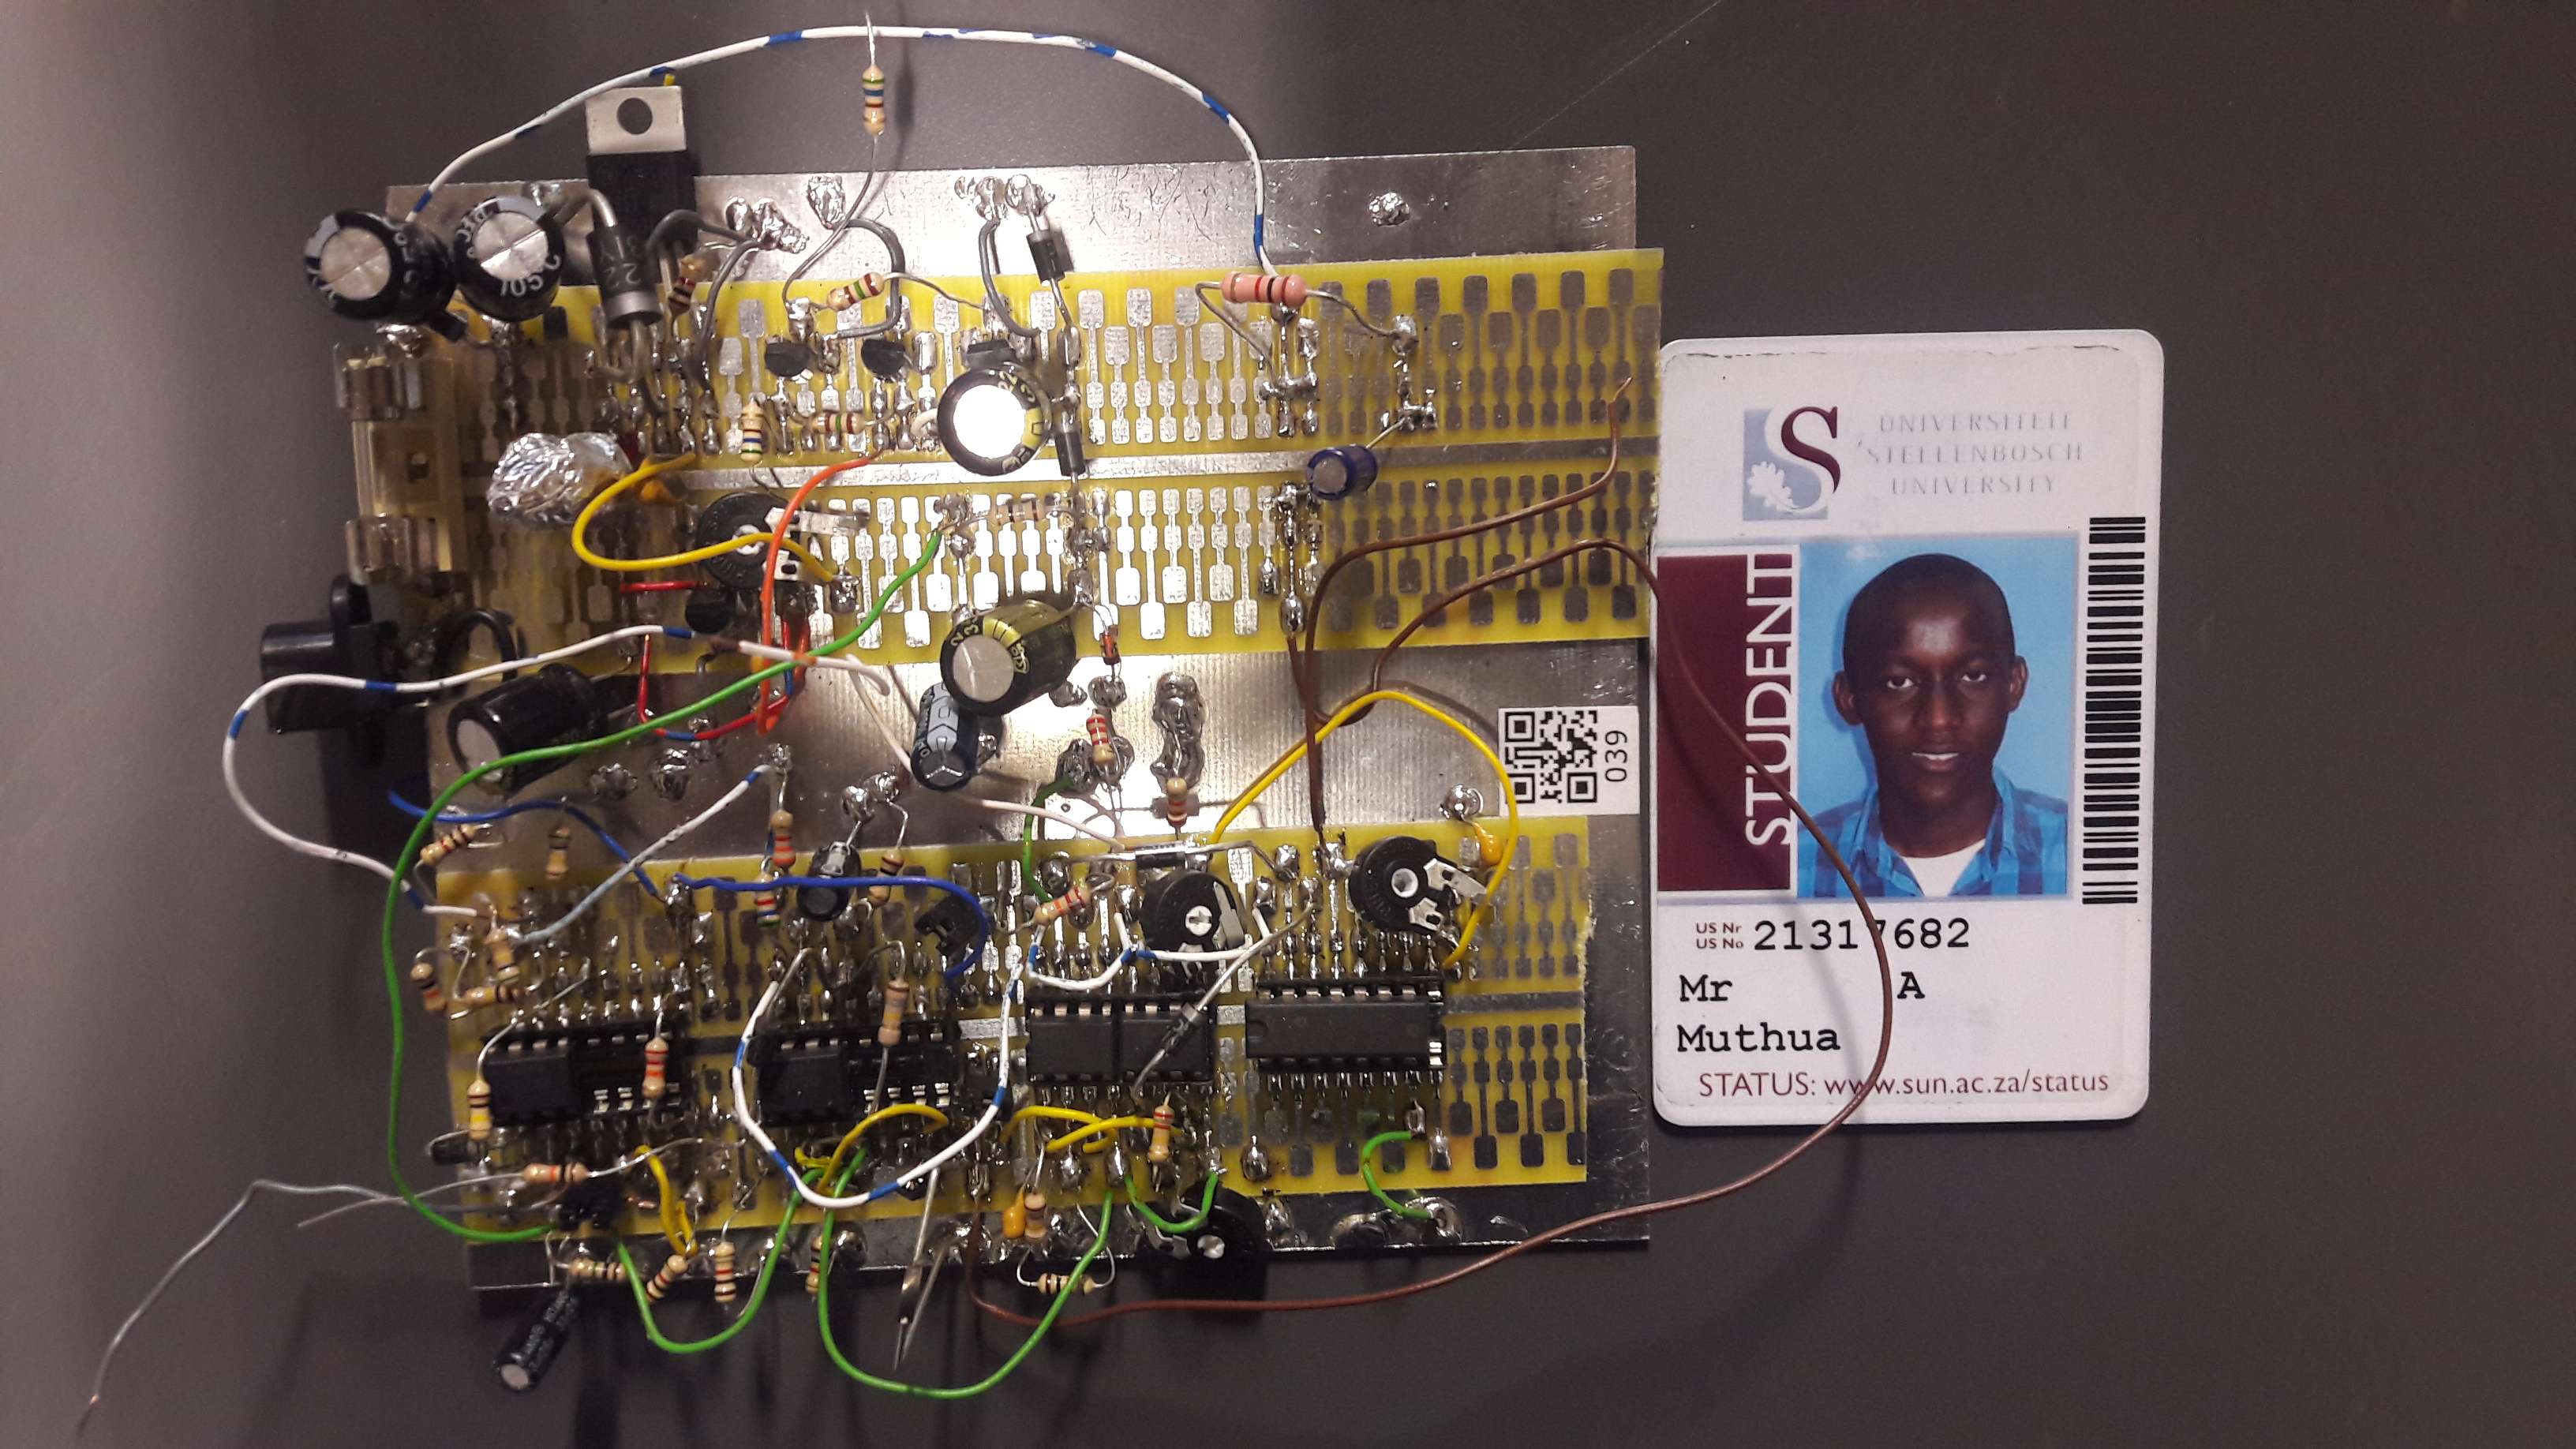
\includegraphics[width=0.5\linewidth]{./Figures/Assignment2_PCB}
		    \caption{Assignment 2 PCB.} \label{fig:pcb}
 \end{figure}
 
 \begin{figure}
 \centering
     \begin{subfigure}[]{0.35\textwidth}
        \centering
         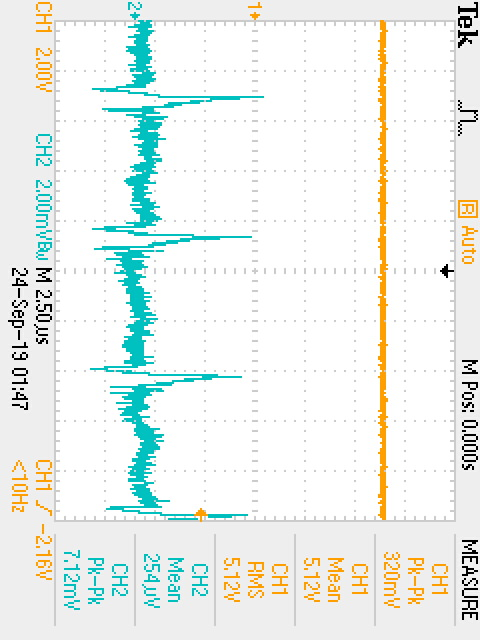
\includegraphics[height=1\linewidth, angle=90]{./Figures/+5V}
		    \caption{+5V rail with noise level.} \label{subfig:+5v_rail}
     \end{subfigure}
      \begin{subfigure}[]{0.35\textwidth}
              \centering
  		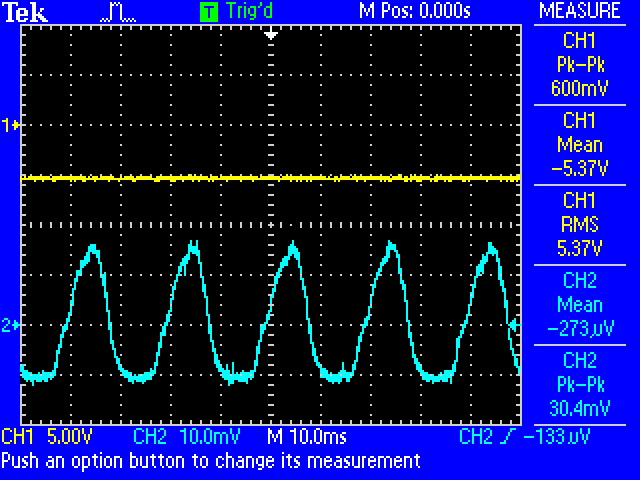
\includegraphics[width=1\linewidth]{./Figures/-5V}
		    \caption{-5V rail with noise level.} \label{subfig:-5v_rail}
     \end{subfigure}
   \caption{Noise and rail voltages with all three systems running together.}
    \label{fig:rails}
 \end{figure}
 
 
By using a multimeter in series with both the +5V and -5V supply, it is measured that the system draws $\SI{8.38}{\milli\ampere}$ from the +5V supply and $\SI{6.84}{\milli\ampere}$ from the negative rail. This is lower than the estimation in Section \ref{sec:system}.











\appendix%===========================================================


\backmatter%=========================================================

\bibliography{References}
\renewcommand{\thesection}{A.\arabic{section}}
\renewcommand{\thechapter}{A.}
\begin{appendix}

     \chapter{Appendix A: Social contract}
     \vspace{-15mm}
     \begin{figure}[!htb]
     \centering
     	\fbox{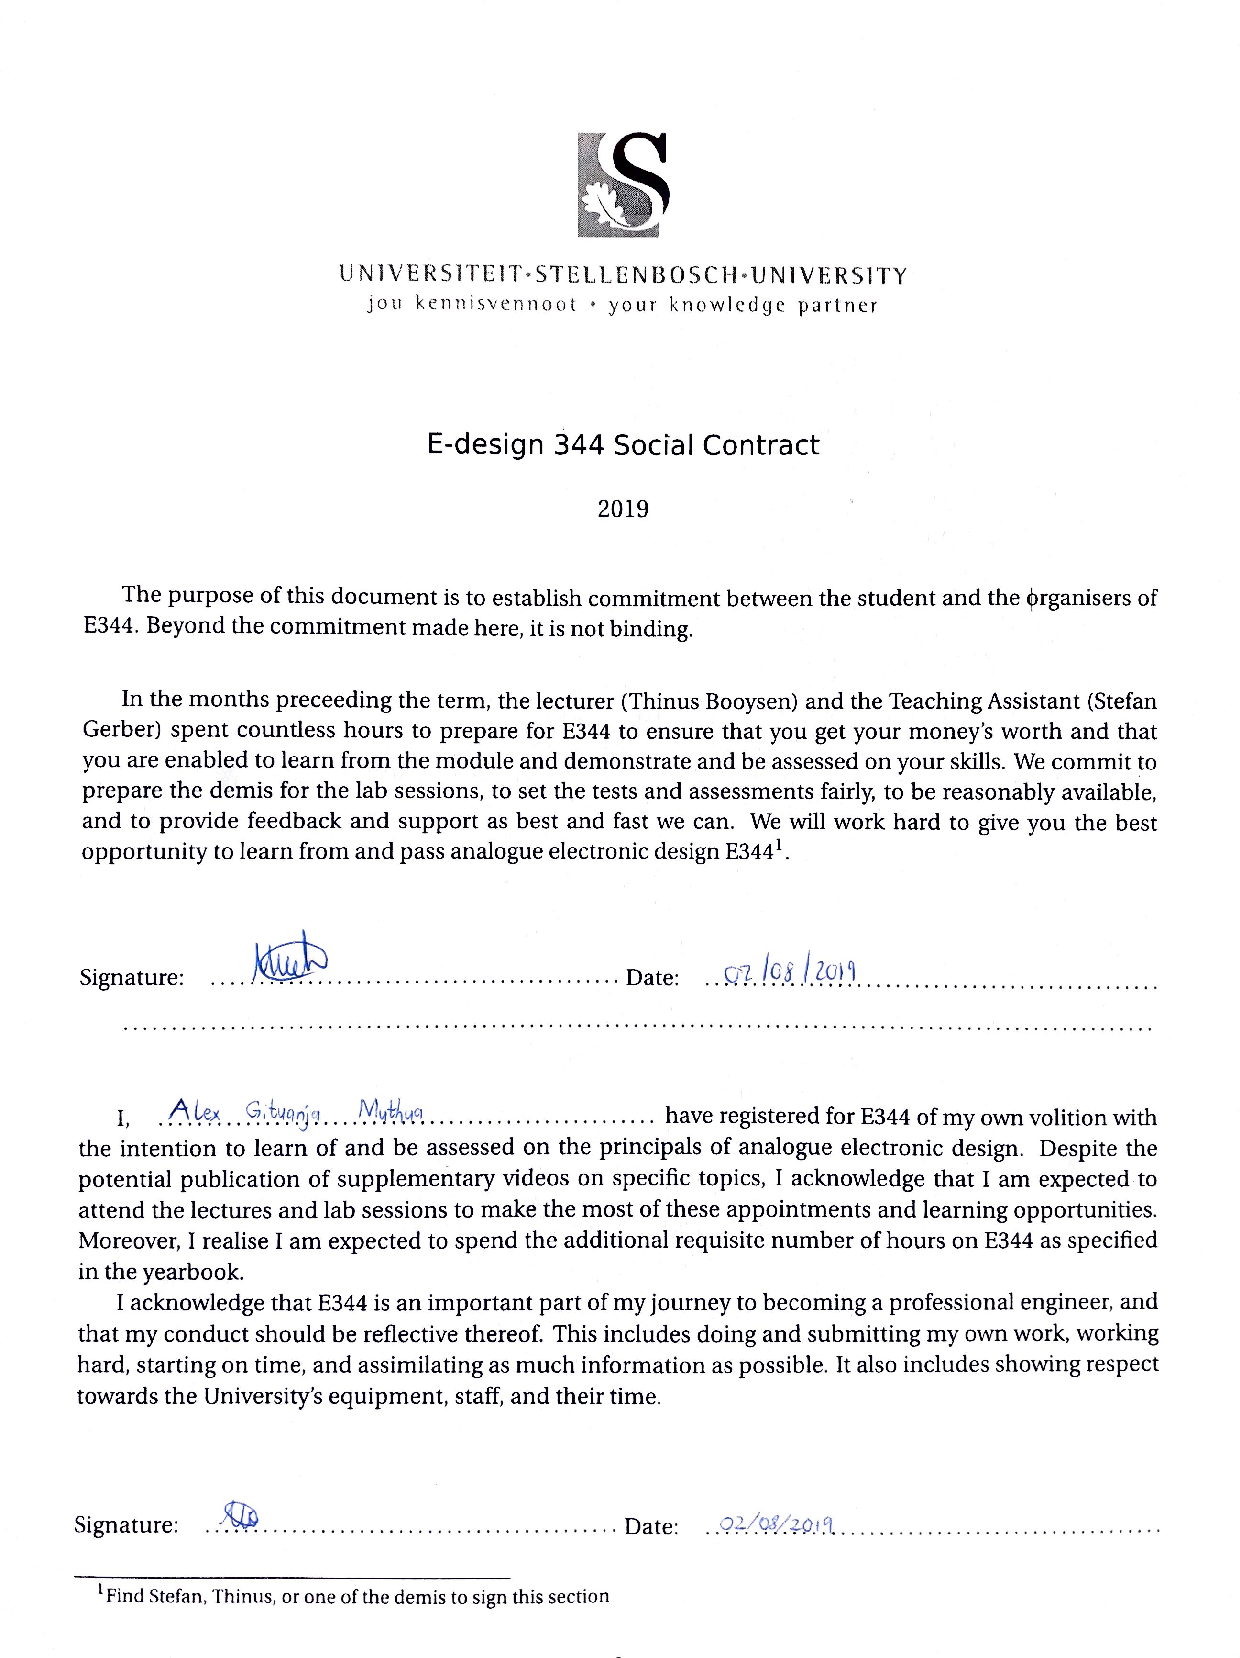
\includegraphics[width=0.78\linewidth]{./Figures/social_contract.pdf}}
       \label{fig:social_contract}
	\end{figure}
     \chapter{Appendix B: Wiring safety check}
     \vspace{-15mm}
     \begin{figure}[!htb]
     \centering
     	\fbox{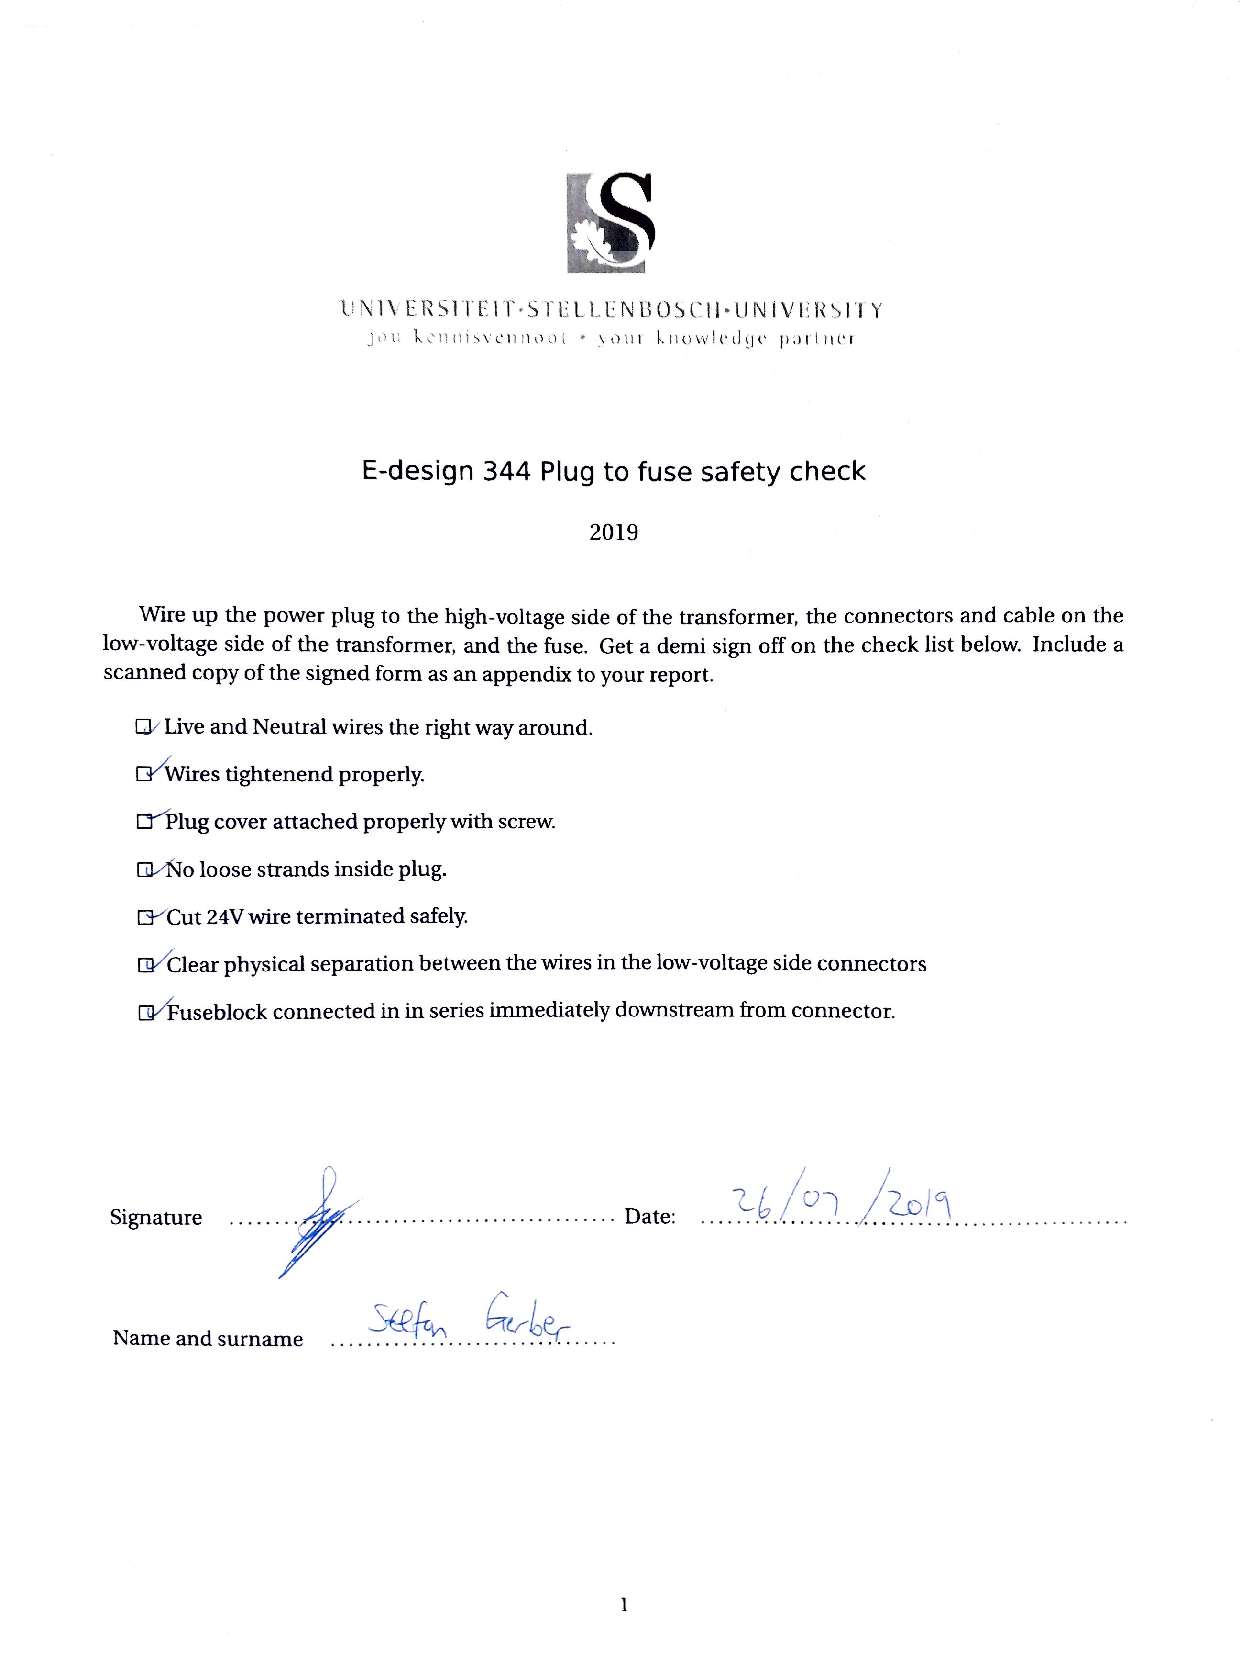
\includegraphics[width=0.78\linewidth]{./Figures/safety_check.pdf}}
	\label{fig:plugSafety}
	\end{figure}
     \chapter{Appendix C: Screengrab of GitHub repo}
     \vspace{-15mm}
     \begin{figure}[!htb]
     \centering
     	\fbox{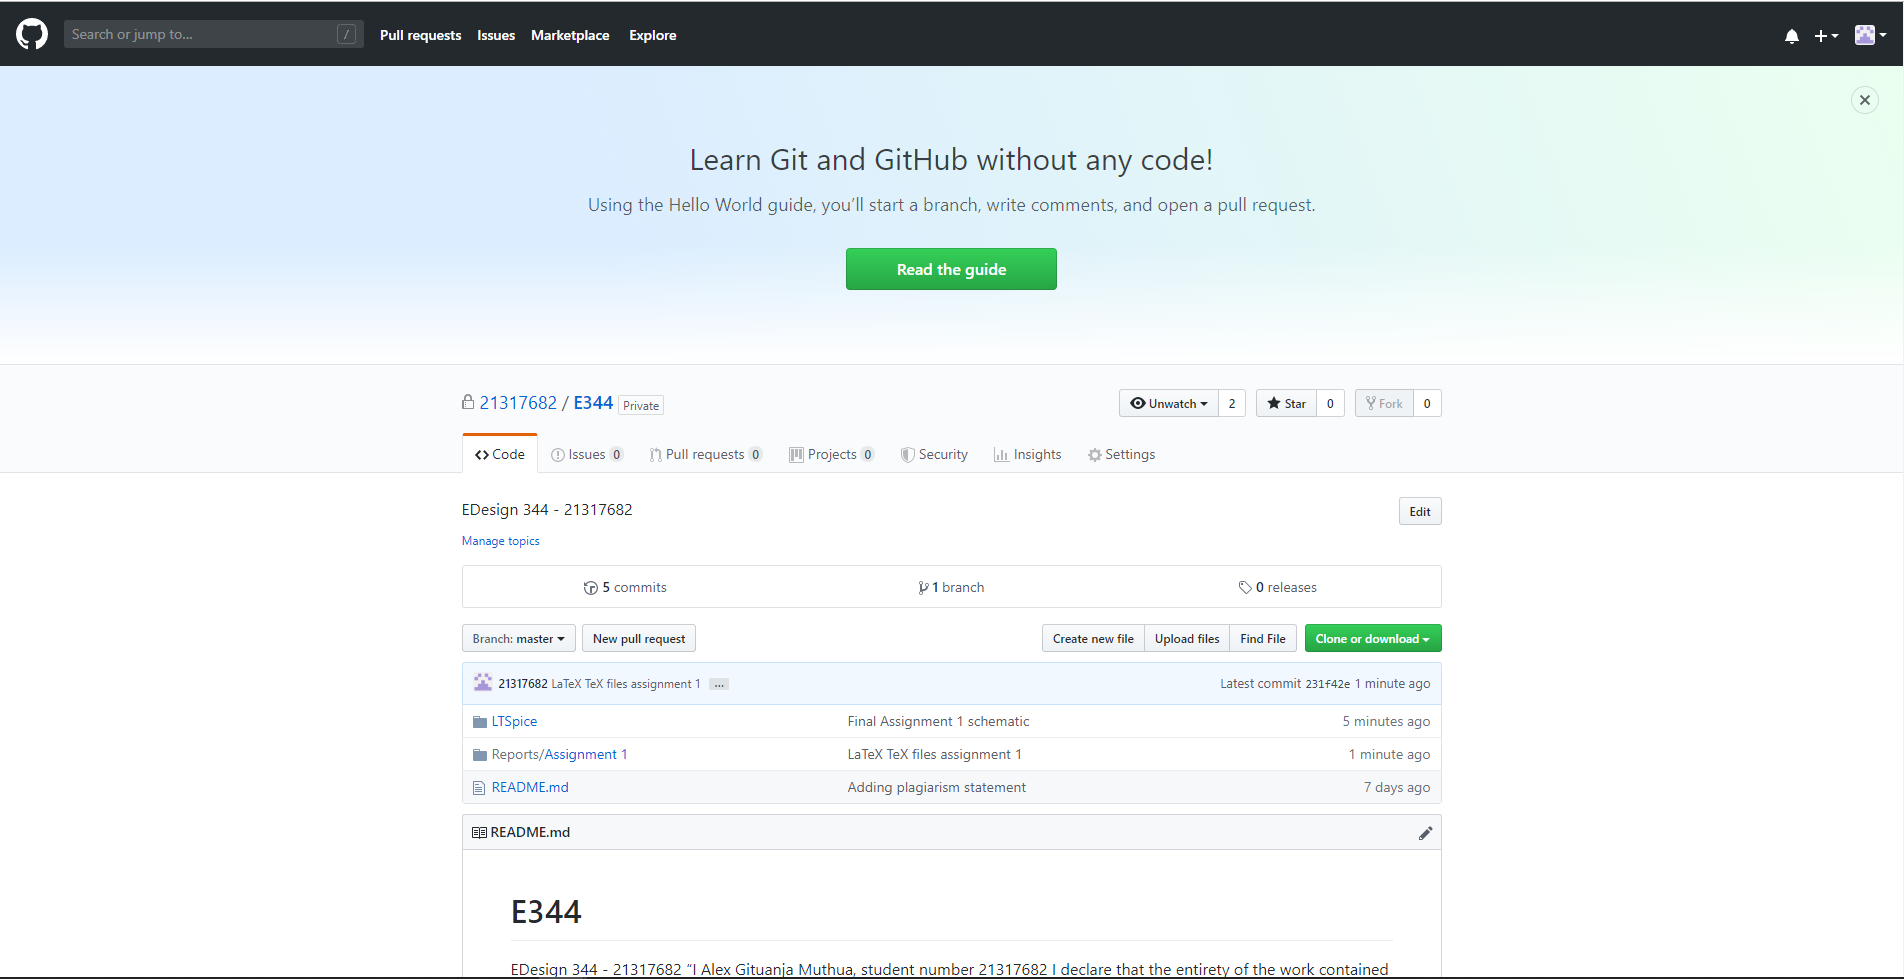
\includegraphics[width=0.98\linewidth]{./Figures/github_repository_A1}}
	\label{fig:github}
	\end{figure}
\end{appendix}
\end{document}
